%# -*- coding:utf-8 -*-
\chapter{基于CTA的冠状动脉的分割与可视化}
\label{chap5}

\section{Introduction}

Coronary artery diseases are one of the key causes of deaths in the modern world. % \cite{WHO2013}.
The fatty blood clot (or plaque) adhering to the inner wall of the tiny vessels can partly or completely block the supply of oxygen and other nutritious substances for the heart muscles.
The diseases may lead to serious or even fatal health problems, such as angina and heart attack \cite{OCallaghan2002}.
%The unhealthy living habits have been proved to be the main reasons that cause the fatal diseases \cite{Go2013}.
Percutaneous coronary intervention (PCI) is the standard clinical solution to the coronary heart diseases.
Comparing with the traditional paradigm of the thoracic surgery, this procedure causes much less incisions and trauma, shorter operation time and post-op observation.
Therefore, this skill lies at the core place in the toolkit of a cardiologist.
Regarding the minimally invasive feature of PCI, the clinicians need to master the insight of the complicated anatomic structures of the coronary arteries and the manipulation of the tools.
Moreover, they must conquer the difficulties of the coordination between eyes and hands during the procedure \cite{Li2012CUHK}.
However, risks arise.
Instances are orthopedic injuries turn out due to the prolonged standing and the heavy weight of the lead protection apron during the PCI procedure \cite{Goldstein2004}, and high incidence rate of brain tumors caused by the long-term ionizing radiation under the fluoroscope \cite{Roguin2012}.

To gain the mastery of this important and complex technique, one must endure sufficient and strict drills under the supervision of the mentor before his/her solo surgery.
Most of the medical institutions and hospitals used to train their residents/interns who aim to be a cardiologist mainly based on human cadavers and living animals \cite{Lunderquist1995}, as well as non-biological models \cite{Mori1998}.
Although these training methods successfully protect the trainees from the common occupational hazards, they also have their flaws:
there is no blood circulation in the human cadavers;
the animal's anatomic structures are different from the human's;
and the preservation of the cadavers and the raising of the animals cost a lot of money and all of them cannot be reused.
The physical models need to be routinely maintained and have limited lifetime, despite they can provide intuitive appearance of the human body.

Computer-aided surgical simulation demonstrates its unique characteristics, such as radiation-free, rich details of the procedure-related anatomy, schedule-free, and ease of maintain.
Numbers of simulation systems were developed in research institutions \cite{Dawson1996DK,Wang1997ICard,Cotin2000ICTS} and technological incorporations \cite{CAEWeb,MenticeWeb,SimbionixWeb}.

Intravascular surgical robots provide the cardiologists brand-new facilities to perform the PCI procedures \cite{NIOBEWeb,HansenWeb,Beyar2006RNS,Smilowitz2012}.
Since the manipulation of the robots are different from the traditional procedure, one needs to learn and practice in a series of lessons.
In this training process, new problems emerge.
First, training on the real robot systems is a huge waste of high-end medical resources.
Second, the robotic training shares the same problems with its traditional counterparts.
Robotic surgical simulation for the da Vinci system have proved successful in solving the problems \cite{Liss2012,Kesavadas2011}.

The aim of this work is to develop an approach to visualize the coronary arteries based on the computed tomography angiography (CTA).
The acquired model will be the critical part of the blood vessel model in the robotic intravascular surgical simulator designed for the robot-assist intravascular surgical system \cite{Ji2011EMBC}.
The segmentation of the coronary vasculature is a difficult and demanding work.
Due to their tiny scale and complex topology, the coronary arteries in CTA are often in relatively low intensities and the complicated details may get lost during the processing.
To address this problem, an approach based on the multi-scale tubular enhancement and an improved geodesic snakes is designed.
For a better segmentation, the vessels are enhanced at first.
The pixels are convolved with a Gaussian kernel to compute the Hessian matrix.
Then we take the eigenvalues of the matrix to calculate the ``vesselness" measure.
Next the speed images are generated by computing gradient and applying nonlinear intensity mapping to the enhanced images.
Simultaneously the initial level sets are generated by the improved fast marching algorithm.
After the above computation complete, the actual fronts propagation starts and the final segmentation results are conversed after the propagation ends.
Then the visualization model of the coronary arteries are extracted.
The experimental results demonstrate that the approach is capable of visualizing the coronary arteries in the CTA.

The rest of this paper is organized as follows.
Section II outlines the precessing work flow and details the techniques introduced in the segmentation tasks.
Section III describes the experiments and presents the results.
The final section concludes the whole work.

\section{Methodologies}

This section discusses the design of the segmentation pipeline and details the principles of the consisting modules.
Fig. \ref{fig:DataFlow} presents the block diagram of the processing pipeline in the bird's-eye view.
The data type of the pixels in the original images is firstly converted.
After the images are appropriately thresholded, the data needs to be enhanced appropriately, right before sending the data to the downstream modules.
The enhancement should highlight the ``tube-like" objects, which are the coronary arteries in this paper.
Next the intensities of the enhanced objects are tuned for the following processing.
Then two computations are performed simultaneously to generate the speed images and the initial contours for the CURVES system.
After that, the results are fed into the CURVES module, where the actual fronts propagation occurs.
The CURVES system can evolve the input contours with the reference of the speed images until the contours ``touches" the wall of the tiny vessels.
Finally the output contours are extracted and then visualized in the surface rendering way.
\begin{figure}[tb]
\centering
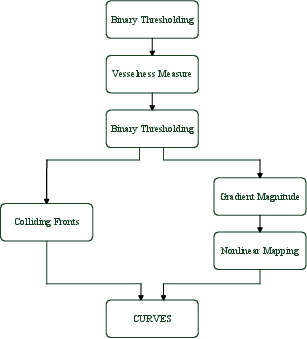
\includegraphics[height=3.2in,width=3.2in]{Figures/DataFlow2.png}
\caption{Collaboration diagram of the segmentation pipeline.}
\label{fig:DataFlow}
\end{figure}

\subsection{Tubular Objects Enhancement}

The tubular enhancement is a sort of multi-scale line filtering, whose scheme can be summarized as the ``tube-like" objects in the image are highlighted whilst the rest are attenuated. %
To achieve this, the three dimensional multi-scale algorithm proposed by Sato \textit{et al.} \cite{Sato1998} is introduced.

To shape the filter response to certain width of lines and suppress the noisy effects, the pixels need to convolving with the second order derivatives of a Gaussian kernel.
This computation is an equivalent to the calculation of the Hessian matrix $\mathcal{H}$ of the three-dimensional image $I(\cdot)$:
\begin{gather}
\label{eqn:Hessian}
\mathcal{H} = \nabla^2 I =
\begin{bmatrix}
I_{xx} & I_{xy} & I_{xz} \\ I_{yx} & I_{yy} & I_{yz} \\ I_{zx} & I_{zy} & I_{zz}
\end{bmatrix},
\end{gather}
where $I_{xx} = \frac{\partial^2 I}{\partial^2 x}$, $I_{xy} = \frac{\partial^2 I}{\partial x \partial y}$, to name a few.
And all these partial second order derivatives are the convolutions with the second order derivatives of a Gaussian kernel $G(x; \sigma)$ with the standard deviation $\sigma$:
\begin{equation}
\label{GaussianConvolution}
I_{xx} = I \ast \frac{\partial^2 G}{\partial^2 x}.
\end{equation}
The eigenvalues of (\ref{eqn:Hessian}) are $\lambda_1$, $\lambda_2$, and $\lambda_3$ with their values in descending order.
Their associated eigenvectors are $e_1$, $e_2$, and $e_3$, respectively.

When $\lambda_1 \approx 0$ and $\lambda_2 \approx \lambda_3 \ll 0$, the line measure can be written as
\begin{equation}
\label{eqn:LineMeasure}
\lambda_{123} =
\begin{cases}
\left| \lambda_3 \right| \left( \frac{\lambda_2}{\lambda_3} \right)^{\gamma_{23}} \left( 1 + \frac{\lambda_1}{\left| \lambda_2 \right|} \right)^{\gamma_{12}}, & \lambda_1 \le 0 \\
\left| \lambda_3 \right| \left( \frac{\lambda_2}{\lambda_3} \right)^{\gamma_{23}} \left( 1 - \alpha \frac{\lambda_1}{\left| \lambda_2 \right|} \right)^{\gamma_{12}}, & \frac{\left| \lambda_2 \right|}{\alpha} > \lambda_1 > 0 \\
0, & \text{otherwise}.
\end{cases}
\end{equation}
In (\ref{eqn:LineMeasure}), the additional parameters $\gamma_{12}$, $\gamma_{23}$, and $\alpha$ are all positive constant, where $\gamma_{12} \in [0, \infty)$ is used to discriminate between the branching structures and the noises as well as pseudo-branches, $\gamma_{23} \in [0, \infty)$ regulates the sharpness, and $\alpha \in (0, 1.0]$ maintains the asymmetrical characteristics of the last terms of the function for all possible $\lambda_1$.

Additionally, different choices of the eigenvalues can equip the line filter with the abilities in detecting different shapes of the objects as shown in Table. \ref{tbl:Eigenvalues}. %

\subsection{Preprocessing for Level Set Evolution}

\subsubsection{Speed Images Calculation}

Level set algorithms evolves the contours in the gradient field with ``sharp" variations in intensity values from the inner or outer area to the boundaries.
The aim of the speed images is to provide this gradient field in the form of nicely shaped gradient images.
In the gradient images, the magnitude of the gradient at each pixel is calculated.
Next the gradient images $I_{\nabla}$ are transformed into the speed images $I_{\sigma}$ by applying the nonlinear relation:
\begin{equation}
\label{eqn:Sigmoid}
I_{\sigma} = (I_{max} - I_{min}) \cdot \frac{1}{1 + \exp\left(-\frac{I_{\nabla} - n}{m}\right)} + I_{min},
\end{equation}
where $I_{max}$ and $I_{min}$ are the two extreme values of the output intensity values, $m$ is a constant that controls the window width of the input intensity, and $n$ is a constant that defines the center of the window.
\begin{table}
\renewcommand{\arraystretch}{1.3}
\caption{Eigenvalue sets for detecting different shapes}
\label{tbl:Eigenvalues}
\centering
\begin{tabular}{l||c}
\hline
\bfseries Shape & \bfseries Eigenvalues \\
\hline\hline
Bright tubes   & $\lambda_1 \approx 0, \lambda_2 \approx \lambda_3 \ll 0$ \\
Dark tubes     & $\lambda_1 \approx 0, \lambda_2 \approx \lambda_3 \gg 0$ \\
Bright plates  & $\lambda_1 \approx \lambda_2 \approx 0, \lambda_3 \ll 0$ \\
Dark plates    & $\lambda_1 \approx \lambda_2 \approx 0, \lambda_3 \gg 0$ \\
Bright spheres & $\lambda_1 \approx \lambda_2 \approx \lambda_3 \ll 0$ \\
Dark spheres   & $\lambda_1 \approx \lambda_2 \approx \lambda_3 \gg 0$ \\
\hline
\end{tabular}
\end{table}

\subsubsection{Initial Contours Evolution Using Colliding Fronts}

The aim of the colliding fronts module is to evolve the contours for the CURVES system from the user-defined seeding points.
The colliding fronts method is implemented based on the principles of the fast marching algorithm \cite{Sethian1999}.
However, this method requires two seeds for each round of evolution such that the area between the seeds can be extracted.
The output of this module is the dot production of the gradient field of arrival times of the two wavefronts.
The level set initialization for the prolonged objects greatly benefit from this feature of the method.
On the other hand, the method also shortens the computation time.

\subsection{CURVES Evolution Model}

The CURVES method \cite{Lorigo2001} is chosen as the functioning segmentation method because of the complex nature of the coronary arteries.
It is highly effective in the segmentation of the complicated curvilinear structures in the volumetric medical images.
In addition, the criterion of CURVES method also takes the local smoothness of the boundaries to be detected (i.e., the inner wall of the coronary arteries) into account.

This method is a modification of the geodesic active contours method developed in Caselles \textit{et al.} \cite{Caselles1997}.
As the extensive research of the geodesic active contours, CURVES is a level set algorithm that models the tiny vessels as spatial curves with arbitrarily complicated topology \cite{Lorigo2001}. %
CURVES evolves the level sets to the boundaries of the targets based on the criterion of the minimization of the following energy functional
\begin{equation}
\label{eqn:CURVES}
\oint_0^1 g\left( \left| \nabla I \left( \mathcal{C} \left(  s \right) \right) \right| \right) \left| \mathcal{C}'\left( s \right) \right| ds,
\end{equation}
where $\mathcal{C}\left( s \right): [0,1] \rightarrow \mathrm{R}^3$ is a one-dimension curve, $I\left( \cdot \right): [0, a] \times [0, b] \times [0, c] \rightarrow [0, \infty)$ is an image on which the curve evolution takes place, and $g\left( \cdot \right): [0, \infty) \rightarrow \mathrm{R}^+$ is a monotonically decreasing function. %

The minimization of this functional can be achieved by searching for the gradient descent direction of the functional itself, which means the Euler-Lagrange equations associated with (\ref{eqn:CURVES}) needs to be computed. %
Thus the geodesic flow equation that controls the contour evolution in this process of minimization can be obtained as follows
\begin{equation}
\label{eqn:Evolution}
\frac{\partial \mathcal{C}}{\partial t} = k \mathcal{N} - \frac{g'}{g} \varPi \left( \mathcal{H} \frac{\nabla I}{ \left| \nabla I \right| } \right),
\end{equation}
where $\mathcal{H}$ is the Hessian matrix of the image $I$, $k$ is the Euclidean curvature, $\mathcal{N}$ is the unit normal vector, $\varPi(\cdot)$ is the projection operator projects the argument onto the normal space. %
The update equation can be obtained as
\begin{equation}
\label{eqn:Update}
\frac{\partial v}{\partial t} = \mathcal{F} \left( \nabla v(x, t), \nabla^2 v(x, t) \right) + \frac{g'}{g} \nabla v(x, t) \mathcal{H} \frac{\nabla I}{ \left| \nabla I \right| },
\end{equation}
where $v(\cdot): \mathrm{R}^3 \rightarrow [0, \infty)$ is the embedding function of the curve $\mathcal{C}$, $\mathcal{F} \left( \nabla v(x, t), \nabla^2 v(x, t) \right)$ is the smaller eigenvalue of the matrix $P_{\nabla v} \nabla^2 v P_{\nabla v}$. %
The matrix $P_q$ is defined as a projector which projects some vector onto the normal plane of vector $q \in \mathrm{R}^3$:
\begin{equation}
\label{eqn:ProjectionOperator}
P_q = I_0 - \frac{qq^T}{\left| q \right|^2},
\end{equation}
where $I_0$ denotes the identity matrix.

By incorporating the speed images $I_{\sigma}$ to the evolution equation (\ref{eqn:Evolution}), the evolution in our case can be obtained as
\begin{equation}
\label{eqn:Application}
\frac{\partial \mathcal{C}}{\partial t} = k \mathcal{N} - \frac{g'(I_{\sigma})}{g(I_{\sigma})} \varPi \left( \mathcal{H} \frac{\nabla I_{\sigma}}{ \left| \nabla I_{\sigma} \right| } \right).%
\end{equation}

\subsection{Surface Rendering}

The surface information is extracted for the visualization by the marching cubes method \cite{Lorensen1987MC}.
Cubes are created based on the input information and are organized into an array structure.
Each cube consists of eight pixels (each four pixels are from a slice).
The index of each cube is labeled by comparing the intensity values of every pixel to the isovalue of the surfaces.
Next the patterns of the intersection between objects and cubes are initially determined based on the triangulated cases.
Then the precise intersection are computed using linear interpolation with the intensity values at each vertex.
The unit normals to the surface are calculated via central differences for the vertices of the cubes.
Finally the generated triangles are ready for the surface rendering.

\section{Experiments and Results}

\subsection{Medical Data and Experimental Setup}

The original chest CTA series was acquired by a 128-slice Siemens SOMATOM Definition Flash CT.
The slice thickness was $0.6 \text{mm}$ and the in-slice resolution was $0.4 \times 0.4 \text{mm}^2$.
Since the work was all on the coronary arteries, the volume contained the whole heart (i.e., ROI, which is the abbreviation of \textit{region of interest}) was cropped from the original data as shown in Fig. \ref{fig:Original}. %

Numbers of experiments were conducted with different sets of parameters to segment the coronary arteries from CTA for the testament of the approach in this paper.
In our case, the original CTA series in DICOM format had been converted to the form of XML first; and the data type of pixels are converted for the incoming computation.
Next the converted data was enhanced by the module which was implemented based on the algorithm developed in \cite{Sato1998}.
Then the tubular enhanced data was send to the following modules to perform calculations of speed image production and input level sets generation.
The two set of the resulting data from the two computation pipelines were transferred to the CURVES module in order to generate the final fronts evolution results.
Finally, the marching cubes method was employed to extract the iso-surface corresponding to the wall of the coronary arteries.
All the experiments were performed on a machine with Intel's 2.83GHz Core 2 Quad CPU and 4GB RAM.

\subsection{Tubular Enhancement and Its Postprocessing}

Before the tubular enhancement started, a global binary thresholding was performed in order to provide the enhancing filter with the focus on the tiny bright tubular objects.
To achieve this, the thresholder was called to trim the irrelevant contents in the images, e.g., dark lung regions with negative intensity values, bright bone regions with large positive intensity values, etc. %
As shown in Fig. \ref{fig:Binary1}, the intensity values of the regions within the interval between the lower threshold and the upper threshold were uniformly assigned a unique intensity value, i.e., $255$ in our case; the intensity values of the rest regions were uniformly assign a zero intensity value. %

Referring to the shape prior guidelines listed in Table. \ref{tbl:Eigenvalues}, the tubular enhancement filter was fed the parameters to detect the bright tubular objects, i.e., coronary arteries. %
Among these parameters, $\sigma$ controls the diameter of cross-section of the tubular objects to be enhanced, $\gamma_{12}$ is the measure of the tube similarity, and $\gamma_{23}$ is used for the recovery of vessel regions with inhomogeneous contrast or intensity loss. %
As shown in Fig. \ref{fig:Vesselness}, the tiny vessels including the coronary arteries and the vessels in lung areas were enhanced with a small $\sigma$ whilst the tubular structures with cross-section diameters larger than this value were not enhanced. %

The intensity values of the enhanced tubular objects were relatively low and scattered in a wide range.
This is a mass for the selection of the intensity value in the following processing steps.
To deal with it and facilitate this situation, some intensity transformation step was needed.
The nonlinear intensity mapping filter and the binary threshold filter were the candidates.

Equation (\ref{eqn:Sigmoid}) showed that the nonlinear intensity mapping transformed the input image into the image with partial enhancement and partial attenuation.
With the well chosen parameters, the intensity values corresponding to the targeting objects in this case were enlarged and the rest part of the images in lower intensities were all depressed as near zero intensity areas. %
Because of the mapping characteristics of the sigmoid functions, the intensity values of the bright tubular structures were not uniformly distributed and stayed at the relatively low levels (see Fig. \ref{fig:Sigmoid}). %
In another test, the binary threshold filter extracted the pixels with the intensities in the specified range and assigned them with a unique large intensity value as discussed above (see Fig. \ref{fig:Binary2}). %
Comparing the result of the two candidates, the binary threshold filter was selected to improve the results of the precedent tubular enhancement filter (see Fig. \ref{fig:DataFlow}). %
\begin{figure}[tb]
\centering
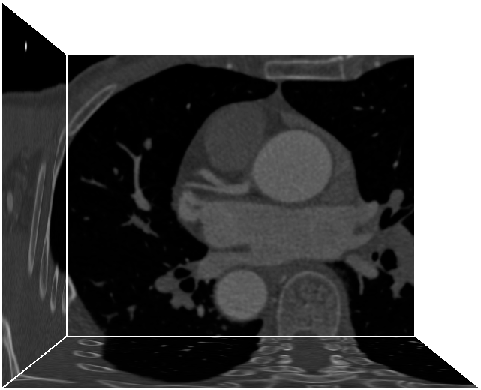
\includegraphics[width=2.8in]{Figures/original.png}
\caption{Original ROI-extracted volumetric data}
\label{fig:Original}
\end{figure}
\begin{figure}[!htb]
\centering
\subfloat{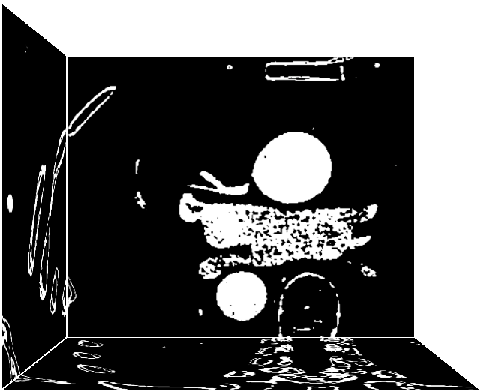
\includegraphics[width=2.8in]{Figures/binary1.png}%
\label{fig:Binary1}}
\hfil
\subfloat{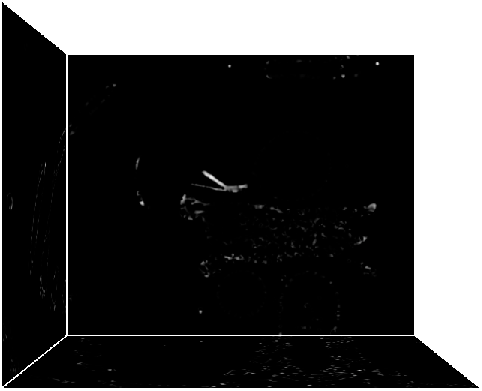
\includegraphics[width=2.8in]{Figures/hessian.png}%
\label{fig:Vesselness}}
\caption{Preprocessing results of the original CTA images based on the ``vesselness" measure: (a) binary thresholding ($\text{lower threshold} = 300$, $\text{upper threshold} = 600$) (b) tubular enhancement ($\sigma = 0.9$, $\gamma_{12} = 0.1$, $\gamma_{23} = 2.0$).}%
\label{fig:Preprocessing}
\end{figure}

\subsection{Feature Images Computation}

To generate the feature images for the CURVES system, two steps were performed:
(1) calculating the gradient magnitude at each pixel; and
(2) converting the gradient images into the speed images.
%\begin{enumerate}
%\item calculating the gradient magnitude at each pixel;
%\item converting the gradient images into the speed images.
%\end{enumerate}
The gradient magnitude module computed the magnitude of the gradient pixel-wisely for the image by performing the convolution with the first order derivatives of a Gaussian kernel.
The wall of the tiny vessels were extracted before the nonlinear intensity mapping was employed to generate the edge potential maps.
The extreme values of the pixel intensities in the gradient magnitude images directly effected the selection of the parameters in (\ref{eqn:Sigmoid}).
To reverse the lightness of the objects (in low intensities in the gradient magnitude images) and its edges (in high intensities in the gradient magnitude images), $n$ was chosen to be the center of the intensity window containing the vessels, and $m$ a negative value with $|m|$ as the width of the window. %
The minus sign of $m$ means the reverse operation on the pixels.
The neighborhood of the boundaries of the objects were in almost zero intensity, which made the evolution driven by (\ref{eqn:Application}) faster in the ``plateau" (with uniformly high intensities), whilst much slower (in a speed of about zero) in the ``ridges" (with rapid decreasing intensities). %

\subsection{Wave Fronts Propagation}

The initial level sets were evolved by the colliding fronts module.
Two seeds were located interior of the regions corresponding to the coronary arteries and the interfaces surrounding each seeds evolved towards each other.
The dot production of the gradients of arrival times of the two wavefronts were computed.
\begin{figure}[!htb]
\centering
\subfloat{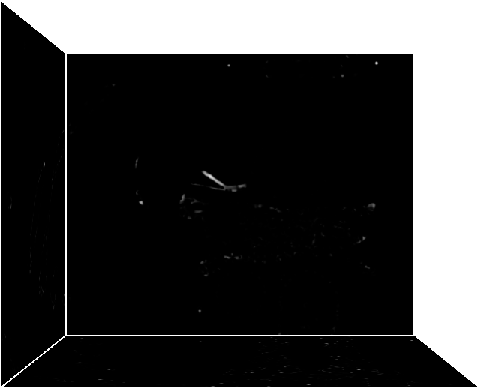
\includegraphics[width=2.8in]{Figures/sigmoid.png}%
\label{fig:Sigmoid}}
\hfil
\subfloat{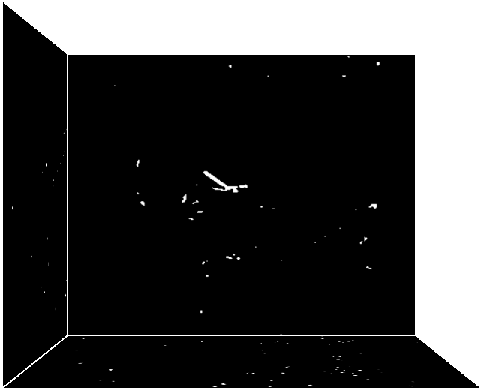
\includegraphics[width=2.8in]{Figures/binary2.png}%
\label{fig:Binary2}}
\caption{Comparison of the two different intensity conditioning approaches: (a) nonlinear intensity mapping ($m = 80$, $n = 120$); (b) binary thresholding ($\text{lower threshold} = 40$, $\text{upper threshold} = 200$).}%
\label{fig:IntensityConditioning}
\end{figure}
\begin{figure}[!htb]
\centering
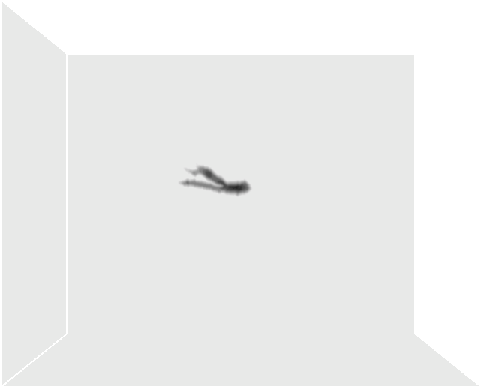
\includegraphics[width=2.8in]{Figures/curves.png}
\caption{CURVES evolution based on the initial contours generated by the colliding fronts method and the edge feature maps calculated by the nonlinear intensity mapping function.}%
\label{fig:CURVES}
\end{figure}
\begin{figure*}[tb]
\centering
\subfloat{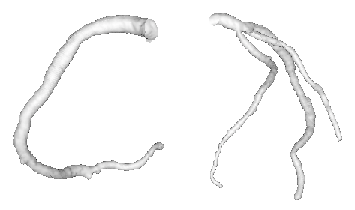
\includegraphics[width=2.8in]{Figures/model_conventional.png}%
\label{fig:VisualizationModelCURVES}}
\hfil
\subfloat{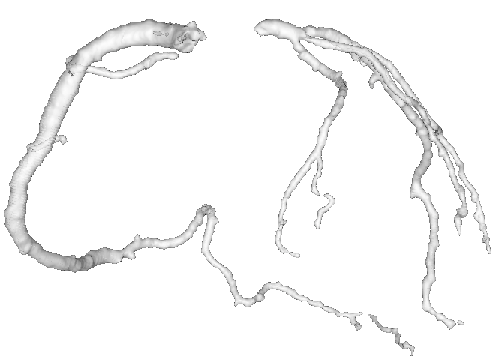
\includegraphics[width=2.4in]{Figures/model_enhanced.png}%
\label{fig:VisualizationModelTECURVES}}
\caption{Models of the coronary arteries: (a) conventional CURVES evolution; (b) tubular-enhanced CURVES evolution.}%
\label{fig:VisualizationModel}
\end{figure*}

The CURVES system started working when all the preceding calculation completed.
The module took the speed images as its evolution maps and the initial contours as its initial states and regulates the evolution according to (\ref{eqn:Application}).
The evolution terminated when the contours evolved against the wall of the coronary arteries in the specified steps of iterations.
And the resulting evolution extracted the coronary arteries as shown in Fig. \ref{fig:CURVES}.
Next a binary thresholding step was provoked to label the inner area of the coronary arteries with high intensity value whilst the outer area with zero intensity value.

\subsection{Visualization of Segmentation Results}

By manually picked the isovalue corresponding to the wall of the coronary arteries, the resulting volume were processed using the marching cubes method \cite{Lorensen1987MC}.
The visualization models of the coronary arteries respectively based on the CURVES regions without and with tubular enhancement demonstrated their capabilities of displaying the complicated geometrical details (see Fig. \ref{fig:VisualizationModelCURVES} and \ref{fig:VisualizationModelTECURVES}). %

\section{Conclusions and Future Work}
%The conclusion goes here.

The three dimensional visualization of the blood vessels plays an important role in the construction of the virtual scenario for the robotic surgical simulator.
Further, the visualization of the coronary arteries is the most critical and difficult work.
Because of the complex spatial topologies, details can be easily lost in the process of segmentation.
In this paper, a vasculature segmentation method based on tubular-enhanced CURVES has been developed.
Then the process of the experiment was presented and the results were demonstrated.
The experimental results showed that the proposed approach is capable of enhancing the tiny dark vessels and visualizing the geometric details of them.

The tubular feature of coronary arteries was enhanced and the speed images were generated.
Meanwhile, the initial contours for the CURVES method were computed by a modified version of fast marching method in another process.
The actual level sets evolution began after the above computation finished and the evolution took a specified number of iterations to detect the coronary arteries.
At the end of the segmentation, the resulting pixels were all conversed in their intensities.
Finally the data representing the surface of the arteries was extracted by the marching cubes method.

Our future plans are the further optimization of the blood vessel models for the simulation with virtual tools of the robotic surgical simulator.
The principle work will be the decimation of the quantity of the triangles consisting the blood vessels and the improvements of the visualization effects of the virtual scenario.